\documentclass[sigconf,nonacm,10pt]{acmart}
\usepackage{lmodern}
\usepackage{amssymb,amsmath}
\usepackage{ifxetex,ifluatex}
\usepackage{fixltx2e} % provides \textsubscript
\ifnum 0\ifxetex 1\fi\ifluatex 1\fi=0 % if pdftex
  \usepackage[T1]{fontenc}
  \usepackage[utf8]{inputenc}
\else % if luatex or xelatex
  \ifxetex
    \usepackage{mathspec}
  \else
    \usepackage{fontspec}
  \fi
  \defaultfontfeatures{Ligatures=TeX,Scale=MatchLowercase}
  \newcommand{\euro}{€}
\fi
% use upquote if available, for straight quotes in verbatim environments
\IfFileExists{upquote.sty}{\usepackage{upquote}}{}
% use microtype if available
\IfFileExists{microtype.sty}{%
\usepackage{microtype}
\UseMicrotypeSet[protrusion]{basicmath} % disable protrusion for tt fonts
}{}
\usepackage{hyperref}
\PassOptionsToPackage{usenames,dvipsnames}{color} % color is loaded by hyperref
\hypersetup{unicode=true,
            pdftitle={Impact of Root DNS Latency on User Experience},
            colorlinks=true,
            linkcolor=blue,
            citecolor=blue,
            anchorcolor=blue,
            urlcolor=blue,
            breaklinks=true}
\urlstyle{same}  % don't use monospace font for urls
\usepackage{natbib}
\bibliographystyle{ACM-Reference-Format.bst}
\usepackage{graphicx,grffile}
\makeatletter
\def\maxwidth{\ifdim\Gin@nat@width>\linewidth\linewidth\else\Gin@nat@width\fi}
\def\maxheight{\ifdim\Gin@nat@height>\textheight\textheight\else\Gin@nat@height\fi}
\makeatother
% Scale images if necessary, so that they will not overflow the page
% margins by default, and it is still possible to overwrite the defaults
% using explicit options in \includegraphics[width, height, ...]{}
\setkeys{Gin}{width=\maxwidth,height=\maxheight,keepaspectratio}
\setlength{\emergencystretch}{3em}  % prevent overfull lines
\providecommand{\tightlist}{%
  \setlength{\itemsep}{0pt}\setlength{\parskip}{0pt}}
\setcounter{secnumdepth}{5}

%\usepackage{caption}
%\renewcommand{\captionfont}{\small} %small fonts for caption
%\renewcommand{\captionlabelfont}{\small}

% \usepackage{url}
% \usepackage{balance}

%% Adding URL breaks
% \makeatletter
% \g@addto@macro{\UrlBreaks}{\UrlOrds}
% \makeatother

% \usepackage{lastpage}

%\usepackage[aboveskip=2pt]{subcaption} %for subfigures

%\setlength{\textfloatsep}{0pt} %spacing between figures and texts
%\setlength{\floatsep}{0pt} 
%\setlength{\dblfloatsep}{0pt}
%\setlength{\dbltextfloatsep}{0pt}
%\setlength{\abovecaptionskip}{0pt}
%\renewcommand{\footnotesize}{\scriptsize}

%\usepackage{etoolbox} % spacing between formula and text
%\apptocmd\normalsize{%
%\abovedisplayskip=0pt
%\abovedisplayshortskip=0pt
%\belowdisplayskip=0pt
%\belowdisplayshortskip=0pt
%}{}{}

%\let\oldfootnote\footnote %small footnote
%\renewcommand{\footnote}[1]{{\oldfootnote{\scriptsize #1}}}


\usepackage{multirow}
\usepackage{graphicx}
%% conference information
% \acmYear{2019}
% \copyrightyear{2019}
% \acmConference{CoNEXT '19}{December 9-12, 2019}{Orlando, Florida, USA}

\hyphenation{name-spaces}

%% System name
\newcommand\thepeering{\textsc{Peering}\xspace}
\newcommand\peering{\textsc{Peering}\xspace}
%\newcommand\peering{\textsc{BGPPlatform}\xspace}
\newcommand\vbgp{\texttt{vBGP}\xspace}
\newcommand\testbed{platform\xspace}
\newcommand\testbeds{platforms\xspace}

%%% Macros for convenience
%% References
\newcommand{\secref}[1]{\S\ref{sec:#1}}
\newcommand{\figref}[1]{Figure~\ref{fig:#1}}
\newcommand{\tabref}[1]{Table~\ref{tab:#1}}
%% to refer to lines in graphs
\newcommand{\linename}[1]{\emph{#1}\xspace}
\newcommand{\parab}[1]{\smallskip\noindent {\bf #1}}

%% Common latin terms
\newcommand{\etc}{\emph{etc.}\xspace}
\newcommand{\ie}{\emph{i.e.,}\xspace}
\newcommand{\eg}{\emph{e.g.,}\xspace}
\newcommand{\etal}{\emph{et al.}\xspace}
\newcommand{\aka}{a.k.a\xspace}

%% editing notes
%\newcommand\ekb[1]{{\color{blue}[ekb: #1]}}
\newcommand\tbd[1]{{\color{red}{\bf TBD: #1}}}
%\newcommand\new[1]{#1}
%\newcommand\cut[1]{}
\definecolor{orange}{rgb}{1.0, 0.31, 0.0}
%\newcommand\edit[2]{#2}
%\newcommand\new[1]{{#1}}
%\newcommand\cut[1]{{#1}}

% terms
\newcommand\noescape[1]{#1}

\newcommand{\rightdownarrow}{\mathrel{\scalebox{1}[-1]{$\Rsh$}}}
\newcommand{\cmark}{\color{green}\ding{51}}
\newcommand{\xmark}{\color{red}\ding{55}}
\newcommand{\metroas}{$\left<\texttt{metro, AS, region}\right>$\xspace}
\newcommand{\fe}{front-end\xspace}
\newcommand{\feplural}{front-ends\xspace}
\newcommand{\capfe}{Front-end\xspace}
\newcommand{\capfeplural}{Front-ends\xspace}

\NewDocumentCommand{\rotseventy}{O{70} O{1em} m}{\makebox[#2][l]{\rotatebox{#1}{#3}}}


% De-Anonymized Commands
\iffalse
\newcommand\ISI{\textsc{the Information Sciences Institute (ISI) at USC}\xspace}
\fi

% Anonymized Commands
\newcommand\ISIone{a research lab in a university in the United States\xspace} % introductory reference
\newcommand\ISItwo{the research lab\xspace} % more general references
\newcommand\ISIthree{a research lab\xspace}

\title{Impact of Root DNS Latency on User Experience}
\author{
            John Heidemann (ISI)
         \and 
            Matt Calder (Microsoft Research)
         \and 
            Arpit Gupta (UCSB)
         \and 
            Ethan Katz-Bassett (Columbia University)
         \and 
            Thomas Koch (Columbia University)
        }
\date{}
\pagestyle{plain}

\begin{document}
\maketitle

\iffalse

subtitle: Paper \#4, \pageref{endofconclusionlabel} pages
(\ref{TotPages} with citations)

classoption: - natbib=true - table header-includes: -
\renewcommand{\shortauthors}{Anonymized} -
\renewcommand{\shorttitle}{User-Perceived Root DNS Latency} -
\setcopyright{none} -
\settopmatter{printacmref=false, printccs=false, printfolios=true} -
\acmDOI{} - \acmISBN{} ---

\fi

\iffalse

Github: https://github.com/tkoch96/root\_dns\_latency Table of contents

\section*{Abstract}\label{abstract}
\addcontentsline{toc}{section}{Abstract}

\section{Introduction}\label{introduction}

\section{DNS -- A Practical Viewpoint}\label{dns-a-practical-viewpoint}

\subsection{Great Latency Savings
Potential}\label{great-latency-savings-potential}

\subsection{Practical DNS Pitfalls}\label{practical-dns-pitfalls}

\section{A Close Look at a Recursive
Resolver}\label{a-close-look-at-a-recursive-resolver}

\section{A Global Look at Users of a Large
CDN}\label{a-global-look-at-users-of-a-large-cdn}

\subsection{Data Sources and
Processing}\label{data-sources-and-processing}

\subsection{Root Latency Experienced by
Users}\label{root-latency-experienced-by-users}

\section{Related Work}\label{related-work}

\section{Conclusion}\label{conclusion}

\fi

\iffalse

Figures to generate: ISI logy root DNS latency MSFT client \# - volume
correlation plot DITL RR query distribution pre and post MSFT join DITL
\& MSFT user latency per day DITL \& MSFT \# user queries per day

Tables to construct: ISI cache hit rate statistics (from Sheet) DITL vs
MSFT vs RIPE matching statistics

\fi

\section*{Abstract}\label{abstract-1}
\addcontentsline{toc}{section}{Abstract}

Anycast is means of distributing content that has been praised for its
simplicity and performance, yet criticized for inflating client
latencies in some cases. The root DNS servers are frequent sources of
information for studies analyzing anycast, since the information is
relatively easy to obtain. We argue that the root DNS servers are not
valid test subjects for studies either offering criticism of or
suggesting improvements for anycast, since clients rarely interact with
the root DNS infrastructure. We demonstrate that simple caching policies
of recursive resolvers limit a clients' exposure to the root DNS
infrastructure, and quantify how much latency a client experiences each
day due to root DNS resolution. These results indicate that future
studies should not draw from root DNS server data to support arguments
regarding anycast latency inflation.

\section{Introduction}\label{introduction-1}

Anycast is a method of server deployment in which a set of physically
distinct servers, called anycast replicas, all serve the same content.
Specifically, IP anycast is a system in which geographically diverse
anycast replicas all advertise the same IP address using the Border
Gateway Protocol (BGP). Routing policies of providers and BGP determine
which anycast replica a client will be mapped to when querying the
(anycasted) IP. This is all transparent to the client, as each site has
exactly the same content.\\
Anycast has been lauded for its potential to offer improved latency and
decreased load on each anycast server, doing so with minimal scaling
complexity. The geographical diversity of anycast deployments offers
resilience to network outages and targeted attacks
\cite{li_levin_spring_bhattacharjee_2018}. However, numerous studies
have argued that anycast can lead to reduced performance for a subset of
clients. Some go further to say that adding more sites may harm, rather
than help user performance. The basic idea behind these claims is that
BGP can sometimes direct clients to far-away anycast servers, despite
the existence of a geographically close server. This inefficiency
unnecessarily inflates latencies for users, and harms their experience.
The root DNS servers notoriously feature in studies involving anycast
because it is relatively easy to gain access to root DNS data,
information about their deployments, and the fact that they are run by
several organizations. This last fact manifests itself in a diverse set
of deployment strategies, for essentially the same service. For example,
in 2018 B-root had 2 server deployments while K-root had close to 70.
These different strategies allow researchers to, for example, coarsely
analyze the effect the number of sites has on the performance of the
service. Using the root DNS servers to draw conclusions about the
performance of anycast as a whole has its drawbacks, as several authors
note. Organizations in charge of managing these services have different
performance goals when deploying new servers. For example, generally,
new root server deployments offer more resilience in the face of attacks
on the DNS infrastructure and so organizations may opt to place their
servers in locations that maximize reachability to at least one replica
in the face of server failure. Conversely, managers of large content
delivery networks (CDN's) may opt to place their servers near large
population centers to provide low latency access to users. This is on
top of the infrastructure the CDN may already have in place, such as a
diverse set of peers or a private wide area network (WAN). Indeed the
everyday notions of ``performance'' that typical users are interested in
are principally important to CDN's, yet only somewhat important to root
DNS managers. Nevertheless, in the face of perceived anycast
inefficiencies many authors have offered solutions ranging from ISP
policy changes to modifications to BGP to bolster the performance of
anycast. Often, studies have framed the problem as a sort of
optimization problem, where every client request should be mapped to the
same physical site as the best unicast alternative. These proposed
modifications are then shown to push anycast closer to optimal
performance. We argue that, in the context of root DNS query resolution,
such modifications and improvements would add negligible benefits to
users. Specifically, we aim to show that the typical user almost never
directly queries the root DNS server. We further place an upper bound on
the amount of latency a typical user of a large CDN experiences each
day, and show that this latency is negligible. In light of these
results, in the context of root DNS anycast deployments, any proposed
improvements for anycast shown to decrease latency for users are of
questionable practical utility. The rest of this paper is organized as
follows. In Section 2 {[}a{]}we provide a description of the DNS
infrastructure as a whole, including some practical details that are
often left out of a routine presentation. In Sections 3 and 4 we attempt
to provide a characterization of how root DNS latency affects the
typical user, from a microscopic and macroscopic viewpoint,
respectively. In Section 5 we discuss related work, and in Section 6 we
conclude our findings.

\section{DNS -- A Practical
Viewpoint}\label{dns-a-practical-viewpoint-1}

Modern day DNS infrastructure is designed so as to limit the time a user
has to wait for DNS query resolution, and specifically root DNS query
resolution.

\subsection{Great Latency Savings
Potential}\label{great-latency-savings-potential-1}

There are many descriptions of DNS and we by no means attempt to give an
introductory lesson. The DNS is a means by which user requests for
human-readable hostnames are mapped to IP addresses. Typically, a user
will send DNS requests in the form of UDP packets to one or more
recursive resolvers (RR's) provided by their
ISP\footnote{ The user can specify whatever RR they wish, but one can sensibly assume the typical user's RR is set by the ISP, broadcasted through DHCP. }.
The RR then requests the records from a root DNS server, top level
domain (TLD) server and authoritative DNS (ADNS) server corresponding to
the record the user requested. Since each request is a correspondence
between the RR and a remote server, there can be several requests made
by the RR for a single user request.

In practice, there is quite a lot of potential for caching these DNS
records, and thus removing unnecessary steps of the recursion outlined
above. Each DNS server provides a time-to-live (TTL) with each record
they return, specifying the duration for which the record can be kept
locally cached. After this duration, the record should be deleted from
the cache of the RR. It has been observed that more heavily accessed
websites tend to purposefully set the TTL of their DNS records to be
some small value, evidence of fine-grained traffic engineering. Hence
the popularity of a website does not make it more likely to live in the
cache of an RR. Nevertheless, RR's can pre-fetch records for popular
websites. For example, a configuration setting on the popular resolver
BIND specifies whether or not BIND should prefetch records set to expire
in a few seconds. In contrast to heavily accessed sites, TLD records
tend to have long TTL's. For example, the COM TLD record (one of the
most popular) has a TTL of 2 days{[}b{]}{[}c{]}. One might speculate
that, since websites users typically access fall into ten or so popular
TLD's, that a request to the root server would rarely occur. In this
scenario, a user fetching example.com would only generate a request for
the COM NS record once every 2 days. Furthermore, some commercial RR's
are known to cache the entire root table locally. Since there are only
1,000 or so TLD's, the memory requirements are quite inexpensive and
caching these records provides huge potential for latency savings. On
top of all of this structure, there can be multiple RR's (a sort of
hierarchy of RR's) among which a query traverses before a third party
(root, TLD, ADNS) is finally queried. This hierarchy compounds the
potential effects of local caching.

Caching at remote RR's is wonderful, and can greatly reduce resolution
time. Indeed since the typical user's RR is run by their local ISP,
generally the user will experience negligible latency for a DNS query if
they hit a warm cache. Modern browsers and operating systems have taken
this one step further and engage in a number of practices that further
aid the user. Operating systems or browsers are known to locally cache
DNS records, as these records are small (compared to say, an image).
Software can go even further, refreshing records in the cache that are
about to expire (just as a RR can do). Features such as link prefetching
in Chrome, where the browser will send DNS requests for all links on a
page, allow the user to completely ``skip'' the DNS resolution process.
All this being said, it is unfortunately quite difficult to quantify the
extent to which these features save users time. Users request web
services through an idiosyncratic combination of browsers, web sites,
operating systems, personalized settings
\footnote{ For example, users can opt out of the link prefetching mechanism in Chrome. },
physical locations, bandwidths, devices, and RR's. On top of this,
everything that has just been mentioned can be undone through poor
configuration or a conservative manager of the RR, as we will now
discuss.

\subsection{Practical DNS Pitfalls}\label{practical-dns-pitfalls-1}

We have discussed the ways in which a user is, by design, prevented from
experiencing latency due to root DNS query resolution. However, there
can be a stark difference between ideal and actual caching behavior.
Although RR's should cache TLD records for the full TTL, unexpected
logical flows in software execution can cause unnecessary queries to the
root server. Furthermore, operators can set conservative settings on the
RR's they run. Regardless of the TTL recommended by the record, the
operator can set this to any value below that recommended TTL.
Furthering the problem, users can disable local DNS caching on their
computers, or use services such as private browsing which disables local
caching for privacy concerns. Web pages can also contain ``hidden'' DNS
requests. The HTTP body of a web page can contain references to
resources stored on third party domains, for which the browser must
request DNS records. Those resources can contain even more references,
creating a chain of DNS requests for potentially uncached records. Users
issuing reverse-DNS lookups or requesting invalid domains always result
in queries to a root server (although it can be argued that these should
not be considered here). Users can also act as their own RR if they
wish, eliminating their ability to leverage the caching capabilities
that are only possible through the ``crowd-sourced'' caching of typical
RR's. Again it is difficult to quantify the degree to which these
pitfalls limit a typical users' ability to leverage the caching
capability of DNS. Notably it is difficult to characterize the
inefficiency introduced by the software employed by the RR of that
users' ISP. One could potentially statistically characterize these
inefficiencies for various open source RR's, which is a subject for
future work.

\section{A Close Look at a Recursive
Resolver}\label{a-close-look-at-a-recursive-resolver-1}

Towards the goal of quantifying the extent to which latency due to root
DNS query resolution impacts the typical user, we analyze packet traces
of a recursive resolver at ISI. The recursive resolver (running BIND 9)
saves all traffic traversing over port 53 to file, and has done so for 5
years, providing us with a rich source of data. This corpus (of users)
is relatively small, and consists of university traffic, so the
specifics of the analysis we conduct may not extend to other RR's.
Nevertheless, we wish to observe some high-level features of the data,
and their implications. We analyze packet traces from the entire month
of January, 2018
\footnote{ The same analysis for the months of May and October [d][e]resulted in the same conclusions }.
We would like to quantify the effect caching root DNS records has on
users, and how this differs from the ideal behavior users can
experience. Specifically, we are interested in the number of queries to
the root server as a fraction of user requests to the recursive
resolver.

\begin{table}[]
\centering
\resizebox{.45\textwidth}{!}{%
\begin{tabular}{lll}
                                                             &                                                                                                                           &                             \\ \hline
\multicolumn{1}{|c|}{\multirow{3}{*}{\textbf{Assumptions}}}  & \multicolumn{1}{l|}{Web Page Load Time (ms)}                                                                              & \multicolumn{1}{l|}{1,000}  \\ \cline{2-3} 
\multicolumn{1}{|c|}{}                                       & \multicolumn{1}{l|}{Root DNS Latency (ms)}                                                                                & \multicolumn{1}{l|}{500}    \\ \cline{2-3} 
\multicolumn{1}{|c|}{}                                       & \multicolumn{1}{l|}{\begin{tabular}[c]{@{}l@{}}Number of DNS Look-Ups \\ Per Web Page\end{tabular}}                       & \multicolumn{1}{l|}{10}     \\ \hline
\multicolumn{1}{|l|}{\multirow{2}{*}{\textbf{Statistics}}}   & \multicolumn{1}{l|}{Number of Client Queries (millions)}                                                                  & \multicolumn{1}{l|}{14.9}   \\ \cline{2-3} 
\multicolumn{1}{|l|}{}                                       & \multicolumn{1}{l|}{Number of Root Transactions}                                                                          & \multicolumn{1}{l|}{73,200} \\ \hline
\multicolumn{1}{|l|}{\multirow{3}{*}{\textbf{Implications}}} & \multicolumn{1}{l|}{\begin{tabular}[c]{@{}l@{}}Percent of Client Queries \\ Resulting in a Root Transaction\end{tabular}} & \multicolumn{1}{l|}{.49}    \\ \cline{2-3} 
\multicolumn{1}{|l|}{}                                       & \multicolumn{1}{l|}{\begin{tabular}[c]{@{}l@{}}Expected Speed-up in PLT with \\ No Root Latency (ms)\end{tabular}}        & \multicolumn{1}{l|}{24.5}   \\ \cline{2-3} 
\multicolumn{1}{|l|}{}                                       & \multicolumn{1}{l|}{Resulting PLT Speedup (percent)}                                                                      & \multicolumn{1}{l|}{2.45}   \\ \hline
\end{tabular}%
}
\caption{Statistics gathered from the ISI RR for the month of January, 2018, and implications of these statistics assuming conservative values for web page load time (PLT), root DNS latency, and number of DNS lookups per page. }


\label{tab:isi_cache_hit_rate_stats}
\end{table}

Relevant statistics and their implications on user-perceived latency are
presented in Table \ref{tab:isi_cache_hit_rate_stats}. Notably we find
that, on average, a user request generates a query to the root server
about .5\% of the time. To obtain an upper bound on the impact of root
latency, assume (conservatively) that a web page load takes 1 second,
that there are 10 serial DNS requests per page, and that the root
latency is 500ms
\footnote{ According to [http archive], and RIPE Atlas, these are quite conservative estimates. }.
The numbers used here are only exaggerated upper bounds on the impact of
root DNS latency, and are only meant to provide context. Supposing root
latency is completely removed from the equation a user saves, on
average, 27 ms per page load. As a percentage of the total page load
time, this is 2.7\%, which is measurable, but not significant. To
provide a sort of visual context for these results, Figure
\ref{fig:isi_root_dns_latency} shows a CDF of root DNS latency
experienced for queries over the same one month period. Requests that do
not generate a query to a root server are counted as having a latency of
0.

{[}f{]}

\begin{figure}
    \centering
    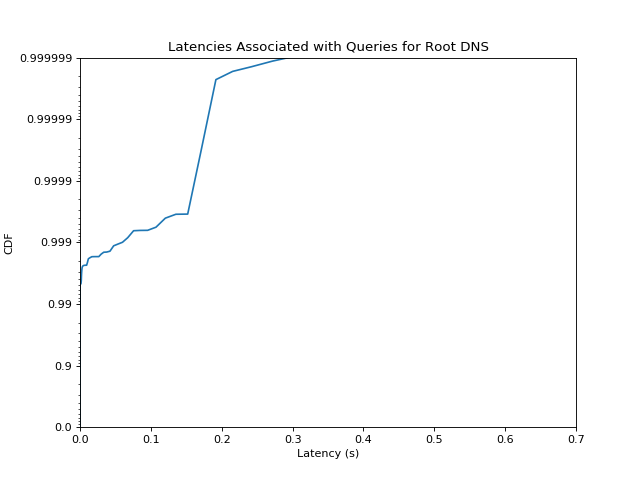
\includegraphics[width=0.45\textwidth]{figures/isi_root_dns_latency.png}
    \caption{Root DNS latency for queries made by clients of the ISI recursive resolver during January, 2018. Client queries that did not generate a query to a root server were given a latency of 0. }
    \label{fig:isi_root_dns_latency}
\end{figure}

Clearly the impact of root DNS latency in this situation is minimal, and
we can reasonably conclude that members of the ISI community do not
experience much latency due to the root DNS servers. However, the impact
on user performance is not as small as one would expect. For example, a
particular day during January 2018 saw as many as 900 queries to the
root server for the COM NS record. Given the 2 day TTL of this record,
this query volume is absurd. This suggests that heuristic arguments that
users rarely experience root latency because cached TLD records have
long TTL's are not sufficient. Manual inspection of specific query
chains in the packet traces suggests that certain logical flows in BIND
can result in the root server being unnecessarily queried. We are not
making claims that BIND has pathological bugs, since we did not explore
the issue further. However, this is an interesting area for future work.

\section{A Global Look at Users of a Large
CDN}\label{a-global-look-at-users-of-a-large-cdn-1}

Looking at cache hit rates of individual RR's is informative, yet does
not provide us with a notion of how much latency each user experiences
in a day. Indeed it would be ideal if we could measure the number of
active clients, how many times those clients request web pages and the
cache hit rates of the clients' recursive resolvers to obtain an
estimate of the latency they experience due to root DNS resolution.

\subsection{Data Sources and
Processing}\label{data-sources-and-processing-1}

Motivated by this ideal scenario, we obtain statistics from a large CDN
operator containing information about the users of that CDN.
Specifically, these statistics include RR IP's, the number of distinct
client IP's behind those RR's and the relative query volume those client
IP's contributed (as a fraction of the total CDN query volume{[}g{]})
for 8 consecutive days in 2019. Working with the notion of a ``user'' is
valuable, as this provides us with an estimate of how much latency each
user experiences. However, since the notion of `user' is an IP address,
one `user' can actually refer to several people behind a NAT.
Furthermore, when weighting results, client query volume is intuitively
the correct metric to weight by, since query volume indicates activity
on the web. {[}h{]}{[}i{]}The relationship between daily average query
volume and daily average client IP count per RR is shown in Figure
\ref{fig:query_client_relationship}. The correlation coefficient between
average weekly volume and client count is .81, with actual daily
correlations ranging from .76 to .85. This correlation is not perfect,
but good enough for us to represent the ``importance'' of an RR by the
number of distinct client IP's behind it.

{[}j{]} query\_client\_relationship

\begin{figure}
    \centering
    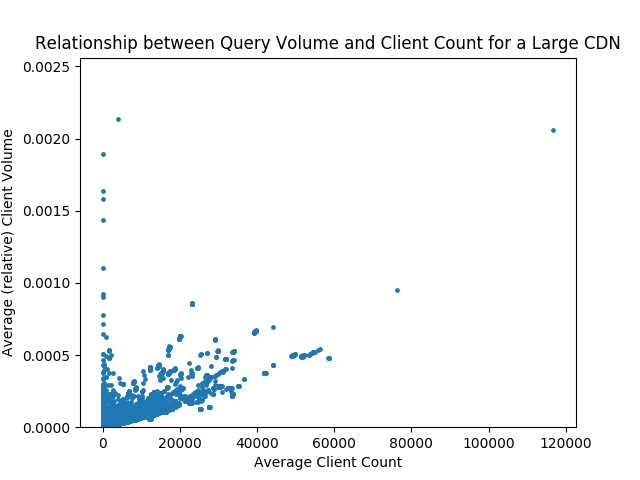
\includegraphics[width=0.45\textwidth]{figures/query_client_relationship.png}
    \caption{Relationship between daily average client count and daily average (relative) query volume for users of a large CDN. Each point represents one RR.}
    \label{fig:query_client_relationship}
\end{figure}

To leverage this CDN data in our aforementioned goal, we augment it with
traces from the 2018 Day in the Life of the Internet (DITL), organized
by OARC. DITL (run annually) contains concurrent packet captures from
all root servers except for G-root
\footnote{ A small portion of data from the 2018 DITL is missing or anonymized. We do not compensate for this, as the impact on the results is likely small. }
for two days in Spring. From DITL, we extracted the frequency of
requests each RR made to each root.

ditl\_volume\_comparisons

\begin{table}[]
\centering
\resizebox{.45\textwidth}{!}{%
\begin{tabular}{|l|l|l|}
\hline
\textbf{Data Set}                            & \textbf{Statistic} & \textbf{Percent Representation} \\ \hline
\multirow{4}{*}{DITL $\cap$ CDN}             & DITL RR's          & 7.2                             \\ \cline{2-3} 
                                             & DITL Volume        & 45.9                            \\ \cline{2-3} 
                                             & CDN RR's           & 87.7                            \\ \cline{2-3} 
                                             & CDN Volume         & 88.9                            \\ \hline
\multirow{4}{*}{DITL $\cap$ CDN $\cap$ RIPE} & DITL RR's          & .1                              \\ \cline{2-3} 
                                             & DITL Volume        & 14.4                            \\ \cline{2-3} 
                                             & CDN RR's           & .9                              \\ \cline{2-3} 
                                             & CDN Volume         & 53.9                            \\ \hline
\end{tabular}%
}
\caption{Statistics displaying the extent to which the RR's of users in a large CDN represent RR's seen in the 2018 DITL captures. Further, it shows the extent to which RR's of RIPE probes represent the 2018 DITL captures.}
\label{tab:dataset_matching_statistics}
\end{table}

We then join these data sets by /24, aggregating their respective client
IP counts, query {[}k{]}volumes, etc\ldots{} -- this joined data set is
referred to henceforth as the DCDN data set. Naturally, there is a
mismatch in the /24's represented by each data set. Table
\ref{tab:dataset_matching_statistics} summarizes the extent to which the
DCDN data (which is a subset of all users) represents the DITL captures,
and vice versa. We also henceforth refer to these /24's as RR's, even
though each data point may represent several RR's. Although the DCDN
data considers a relatively small percentage of all RR's, it captures a
disproportionately large amount all DITL volume. A useful visualization
of the effect of removing these RR's from consideration is shown in
Figure \ref{fig:ditl_volume_comparisons}. The quartiles of the DCDN
volume counts (blue) are approximately 10-times those of DITL (orange),
suggesting /24s in the DCDN particularly active subset of all RR's. This
suggests that, despite disregarding many RR's, our analysis actually
provides an upper bound on root DNS latency experienced by the typical
user.

\subsection{Root Latency Experienced by
Users}\label{root-latency-experienced-by-users-1}

Our main result, shown in Figure \ref{fig:user_root_latency_per_day}, is
a CDF of expected user latency per day, where the expected value is
calculated according to certain assumptions we make about root latency.
We have also included the number of requests each user makes per day in
Figure \ref{fig:user_num_requests_per_day} for reference. Figure
\ref{fig:user_num_requests_per_day} may be particularly useful for
comparing these results with other studies that show CDF's of user
latencies to various roots.{[}l{]}{[}m{]}

user\_root\_latency\_per\_day

\begin{figure}
    \centering
    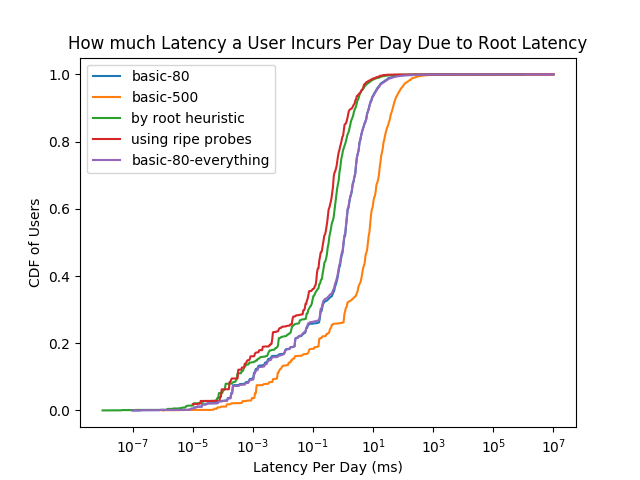
\includegraphics[width=0.45\textwidth]{figures/user_root_latency_per_day.png}
    \caption{A CDF of approximate latency a user experiences due to root DNS resolution, per day.}
    \label{fig:user_root_latency_per_day}
\end{figure}

To generate each line in Figure \ref{fig:user_root_latency_per_day}, the
expected root latency per RR per query is multiplied by the number of
queries per day each RR makes. This is then weighted by user count (from
the CDN data set) and the resulting CDF is calculated. The only question
left to answer is how to calculate the expected root latency per RR. As
a useful comparison, we have included lines labeled ``basic-n'' which
are generated naively assuming the latency from every RR to every root
server is n ms. Similarly, the line labeled ``basic-80-everything'' is
generated further assuming every RR in DITL, but not in the CDN data
set, has one user per day. This line therefore includes information
about every RR seen in DITL and is a complete overestimation of actual
latency experienced by each user; however, the two lines are barely
distinguishable. This is further proof of the representativeness of the
DCDN data set.\\
The line labeled ``heuristic root value'' are calculated as follows:
assume each RR queries the set of roots according to a distribution
\(p_{RR}\), where \(p_{RR}\) is a discrete p.d.f. over the 12 root
servers indicating the probability with which the RR chooses each root
server to query. This p.d.f. is calculated directly from the DITL data.
Next, obtain median latency values to each root (e.g.~from RIPE Atlas)
and call these \(l_{RR}\). Note that, for now, \(l_{RR}\) is independent
of RR. Compute the expected latency from each RR to any root as the dot
product between \(l_{RR}\) and \(p_{RR}\) (i.e.~the expectation of the
latency). Although somewhat imprecise, this method of calculating
latency for each user takes into account that some root servers
generally exhibit lower latencies than others due to investments in
infrastructure
\footnote{ For example, at the time of writing the median latency to B root (3 sites) is 130ms whereas the median latency to F root  (225 sites) is less than 5 ms. }.
Hence, this line can be considered a more reasonable estimate of the
latency users experience due to root DNS resolution. This is
corroborated by the ``middle-of-the-pack'' median and \(95^{th}\)
percentile estimates of .352ms/day and 4.104ms/day, respectively.
Finally, the line labeled ``RIPE'' looks only at those RR's in both the
DITL and CDN data sets housing RIPE probes. RIPE probes routinely issue
ping measurements to each root server and report latency values. From
the preceding paragraph, \(l_{RR}\) is then populated from these
measurements for each RR, and the expected root latency per query is
calculated per RR according to \(p_{RR}\). From Table
\ref{tab:dataset_matching_statistics}, we see that /24's housing RR's of
RIPE probes only account for 14.4\% of the volume in DITL, and less than
.1\% of all /24's; hence, RIPE probes are not representative of the
population as expected. However, for clients in these /24's, this is a
fairly accurate measurement of the expected daily latency due to root
DNS resolution. We see this method provides the lowest median and
\(95^{th}\) percentile estimates of .225ms/day and 4.011ms/day,
respectively. This makes sense, as RIPE probes probably reside in areas
of the world with better connectivity.

Regardless of which method is used to calculate expected latency, users
generally experience median values of \(<\) 1 ms/day while worst case
users generally experience \(<\) 50 ms/day. Even when making the
conservative assumption that every root query from every RR takes 500ms,
95\% of users experience no more than 80ms/day of latency due to root
DNS resolution which is \textit{inconsequential}. Moreover, recall that
the notion of ``user'' here is likely a NAT, representing several users,
and that we do not prune requests unrelated to web traffic (e.g.~PTR
requests) or invalid domain look-ups when parsing DITL traces. This
further establishes that Figure \ref{fig:user_root_latency_per_day} is
to be interpreted as a conservative upper bound of daily root latency
experienced by users. Although it may not be valid to reason about
specific numbers obtained from the above analysis, we can conservatively
say that the typical user hardly ever experiences latency due to root
DNS resolution. Therefore when assessing the utility or performance of
IP anycast, it may not be sufficient or useful to point at a set of root
DNS queries that incurred unnecessarily high latency. As we show here,
users rarely interact with the root DNS infrastructure. Hence the
utility of proposed improvements to IP anycast should not be assessed
using root DNS servers, as the generalization ability of the improvement
to all IP anycast systems is unpredictable.

\section{Related Work{[}n{]}}\label{related-workn}

IP anycast is usually studied in two applications: the root DNS servers
{[}{]}, and CDN's {[}{]}. In addition to these topics, we discuss
studies of popular recursive resolvers, and client-centric measurements
of web latency.

\subsection{Root DNS Anycast
Performance}\label{root-dns-anycast-performance}

The performance of anycast in the context of root DNS is generally
gauged by anycast's ability to balance load among server replicas or
provide low latency to users. Generally, all studies conclude that
anycast successfully balances load, while latency performance depends on
the specific deployment configuration. \cite{moura2016anycast} looks at
a DDoS attack on the root name server infrastructure, and generally
shows that anycast is a good defense mechanism against such attacks. An
earlier study, \cite{sarat2006use} confirms that anycast protects the
root DNS infrastructure against such attacks and, furthermore, that
anycast routes users to an optimal location in most cases.
\cite{de2017anycast} looks at user latency to C, F, K, and L-root and
attributes better performance to good geographic location and peering
strategies. These findings coincide with an earlier study,
\cite{ballani2006measurement}, who conclude the performance of anycast
is intrinsically linked to deployment strategy. Additionally
\cite{de2017anycast} finds that as few as 12 sites can provide ``good''
latency to users. \cite{li_leven_spring_bhattacharjee_2018},
\cite{colitti2006evaluating}, \cite{de2017anycast}, and
\cite{liang2013measuring} are all examples of studies who quantify
latencies to various root servers, and note how these compare to the
(optimal) latency of the closest unicast alternative for the client who
issued the query.

\subsection{CDN Anycast Performance}\label{cdn-anycast-performance}

Some CDN's (e.g.~Cloudflare, Edgecast, Fastly) use IP anycast to augment
their serving infrastructure. When deploying an Anycast CDN (ACDN),
delivering content to users with low latency becomes a high priority, as
there is a large financial incentive to do so. The simplicity of IP
anycast comes at the cost of having coarse grained control over where
client queries land. Shifting client load between nodes during peak
hours, for example, is a challenging problem. As a potential solution,
\cite{flavel2015fastroute} and \cite{alzoubi2011practical} use DNS
redirects at ADNS servers to shift load among anycast nodes, albeit in
slightly different ways. \cite{calder2015analyzing} analyzes what
latency clients are achieving, compared to optimal, when being routed to
anycast nodes and finds that 10\% of clients experience a latency
inflation of at least 100 ms.

\subsection{Recursive Resolvers and the Benefits of
Caching}\label{recursive-resolvers-and-the-benefits-of-caching}

Similar to the RR analysis conducted here, \cite{jung2002dns} looks at
DNS traffic on a small network and notably finds that 16\% of queries
resulted in queries to the root, most of which were for invalid domains.
As this study is quite old, it is no surprise that this rate has
decreased (recall we observed .5\% of queries resulted in queries to the
root) since browser designers and network engineers understand the
importance of caching. \cite{callahan2013modern} also look at a RR
network and analyze statistics of DNS exchanges occurring over it
including DNS transaction latencies. Both \cite{lentz2013d} and
\cite{yu2012authority} look at certain pathological behaviors of popular
recursive resolvers, and the implications these behaviors have on root
DNS load.

\subsection{Web Performance}\label{web-performance}

Although we were unable to find any specific study that looked at how
web performance and root DNS latency were related, there are certainly
studies characterizing web performance. \cite{sundaresan2013web}
characterizes web performance bottlenecks in (at the time) new broadband
networks, and finds that latency is the main bottleneck for PLT when the
user's bandwidth exceeds 16 Mbps. However, the study does not
realistically emulate a page load and, in particular, can not analyze
the effect of having multiple DNS resolutions per page. Similarly,
\cite{asrese2016wepr} analyzes how each step of a page load contributes
to the aggregate PLT using a tool designed in-house. However, unlike
\cite{sundaresan2013web}, they did not conduct a large measurement
campaign and do not include information about multiple DNS lookups per
page. A more recent study, \cite{enghardt2019web} provides a brief
survey of web performance measurement studies and explains why it is
difficult (with current practices) to compare two different studies in
web performance.

\iffalse

(studies looking at anycast in context of root DNS servers) Anycast
Performance, Problems and Potential how many sites are enough? A
measurement based deployment proposal for IP Anycast Evaluating the
Effects of Anycast on DNS Root Nameservers Measuring Query Latency of
Top Level DNS Servers Anycast vs.~DDoS: Evaluating the November 2015
Root DNS Event On the Use of Anycast in DNS (studies looking at anycast
in context of CDN's) fastroute A Practical Architecture for an Anycast
CDN Edgecast paper that hasn't been released yet Analyzing the
Performance of an Anycast CDN (studies looking at recursive
resolvers/caching) (maybe) John's TR of how different resolvers query at
different times On Modern DNS Behavior and Properties DNS Performance
and the Effectiveness of Caching D-mystifying the D-root Address Change
Authority Server Selection of DNS Caching Resolvers{[}o{]} (studies
looking at web performance/how client caching effects it) Measuring and
mitigating web performance bottlenecks in broadband access networks
WePR: A tool for Automated Web Performance Measurement Demystifying Page
Load Performance with WProf{[}p{]} \fi

\section{Conclusion}\label{conclusion-1}

IP anycast has come under attack, with studies showing, for example, how
BGP can naturally route clients to suboptimal anycast instances and
inflate client latencies. Due to the relative availability of root DNS
data and diverse deployment strategies of the root DNS servers, they are
common targets for delineating inefficiencies and suggesting
improvements to IP anycast. We argue not only that the root DNS servers
have different design goals (i.e.~resiliency against attacks) than that
of other anycast services, but also that users rarely interact with the
root DNS infrastructure -- rendering perceived inefficiencies and
proposed improvements to be ill-founded when only tested on the root
DNS. Perhaps simple yet effective ideas such as browser link prefetching
or DNS request parallelization should be expanded and their adoption by
users encouraged, rather than proposed improvements to IP anycast.
{[}a{]}section labels is a better way to go about it maybe {[}b{]}maybe
generate a figure showing a CDF of TTL's of all TLD NS records (pretty
easy to generate) {[}c{]}Would probably need to run BIND locally, and
set myself as my own recursive resolver {[}d{]}has 4x cache hit rate
(far fewer client queries?) {[}e{]}Update: pinged John about it with
more information about when issue occurs {[}f{]}maybe use this as a
p.d.f. for ``amortizing'' the root latency in the table {[}g{]}perhaps
elaborate on what is meant by ``query volume''
{[}h{]}+ethanbkb@gmail.com This is one way I currently use Microsoft's
query volume numbers to justify our results. What do you think? {[}i{]}I
was thinking along the lines of weighting root query cost by query
volume (rather than by ``users''). {[}j{]}y axis needs relabeling
{[}k{]}TODO: comment about removing v6 {[}l{]}For example, people could
look at UMD paper and apply the 95\%-ile latency to all clients and see
implications. {[}m{]}Questionable utility, may be a glut of graphs
{[}n{]}cite more numbers maybe {[}o{]}interesting that in 10 minutes
they observe so many queries for COM TLD yet don't see any issue with
that {[}p{]}Might be an interesting tool to use

\bibliography{bib.bib}

\end{document}
